\documentclass{standalone}
\usepackage{tikz}
\usepackage{amsmath, amssymb}
\usetikzlibrary{arrows.meta, positioning, shapes.geometric, calc, shadows}

\begin{document}
	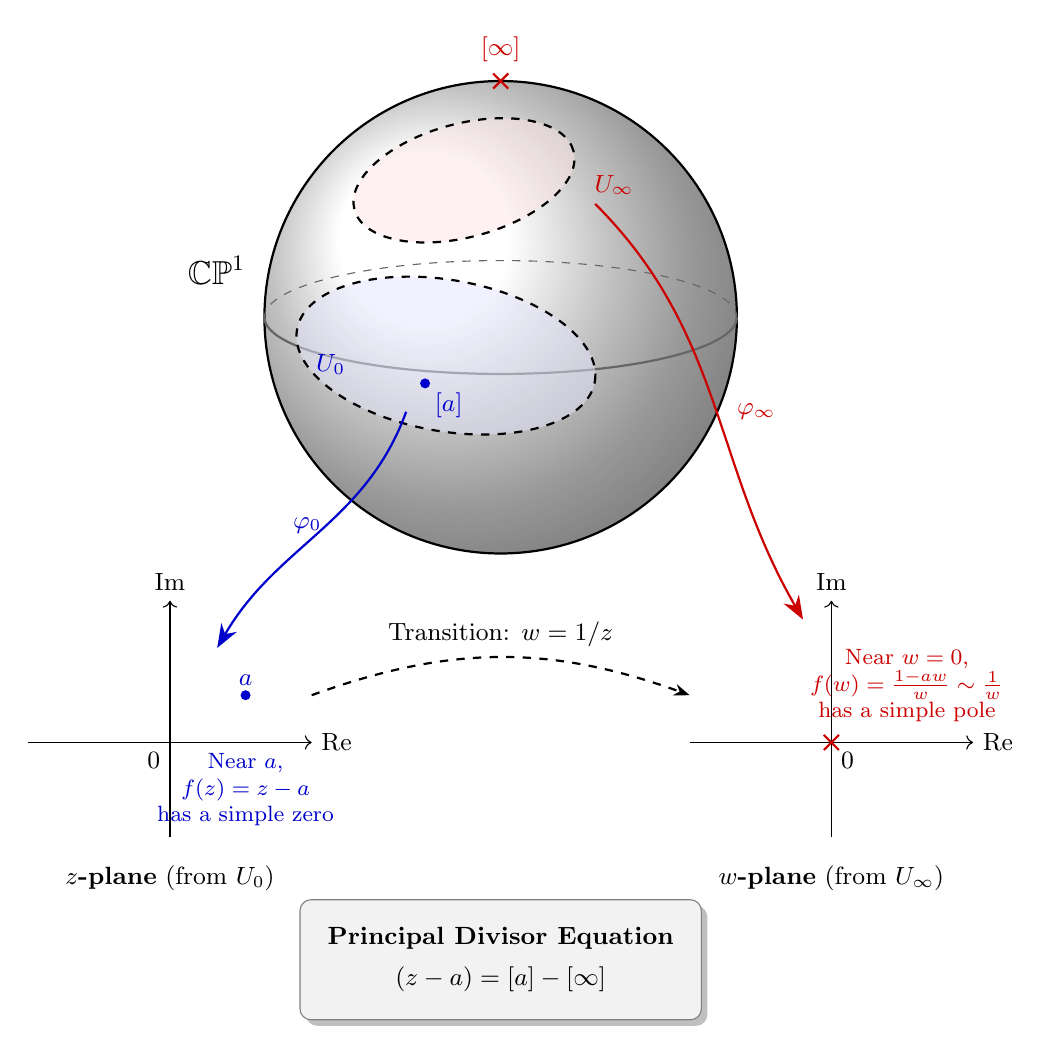
\begin{tikzpicture}[scale=1.2, every node/.style={font=\small}]
		
		% --- Riemann Sphere (CP^1) ---
		% Sphere background with a slight 3D shading
		\shade[ball color=white, opacity=0.8] (0,0) circle (2.5cm);
		\draw[thick] (0,0) circle (2.5cm);
		
		% Equator to give 3D depth
		\draw[dashed, color=black!60] (2.5,0) arc (0:180:2.5cm and 0.6cm);
		\draw[thick, color=black!60] (2.5,0) arc (0:-180:2.5cm and 0.6cm);
		\node[left, font=\large] at (-2.6, 0.5) {$\mathbb{CP}^1$};
		
		% --- Patches on the Sphere ---
		% Patch U_0 (Covers the finite plane, south pole, and equator)
		\draw[thick, dashed, fill=blue!10, fill opacity=0.5, rotate=-10] (-0.5, -0.5) ellipse (1.6cm and 0.8cm);
		\node[blue!80!black] at (-1.8, -0.5) {$U_0$};
		
		% Point a (The simple zero)
		\fill[blue!80!black] (-0.8, -0.7) circle (1.5pt) node[below right] {$[a]$};
		
		% Patch U_\infty (Covers the neighborhood around infinity)
		\draw[thick, dashed, fill=red!10, fill opacity=0.5, rotate=15] (0, 1.5) ellipse (1.2cm and 0.6cm);
		\node[red!80!black] at (1.2, 1.4) {$U_\infty$};
		
		% Point Infinity (The simple pole)
		% Represented with a cross at the North Pole
		\draw[red!80!black, thick] (-0.08, 2.42) -- (0.08, 2.58);
		\draw[red!80!black, thick] (-0.08, 2.58) -- (0.08, 2.42);
		\node[red!80!black, above] at (0, 2.6) {$[\infty]$};
		
		% --- Local Coordinate Planes ---
		% z-plane mapping (bottom left)
		\begin{scope}[shift={(-3.5, -4.5)}]
			\draw[->] (-1.5, 0) -- (1.5, 0) node[right] {Re};
			\draw[->] (0, -1) -- (0, 1.5) node[above] {Im};
			\node[below left] at (0,0) {$0$};
			\node[below] at (0, -1.2) {\textbf{$z$-plane} (from $U_0$)};
			
			% Image of a in the z-plane
			\fill[blue!80!black] (0.8, 0.5) circle (1.5pt) node[above] {$a$};
			\node[align=center, blue!80!black, font=\footnotesize] at (0.8, -0.5) {Near $a$,\\$f(z)=z-a$\\has a simple zero};
		\end{scope}
		
		% w-plane mapping (bottom right)
		\begin{scope}[shift={(3.5, -4.5)}]
			\draw[->] (-1.5, 0) -- (1.5, 0) node[right] {Re};
			\draw[->] (0, -1) -- (0, 1.5) node[above] {Im};
			\node[below right] at (0,0) {$0$};
			\node[below] at (0, -1.2) {\textbf{$w$-plane} (from $U_\infty$)};
			
			% Image of infinity (which is w=0 in this chart)
			\draw[red!80!black, thick] (-0.08, -0.08) -- (0.08, 0.08);
			\draw[red!80!black, thick] (-0.08, 0.08) -- (0.08, -0.08);
			\node[align=center, red!80!black, font=\footnotesize] at (0.8, 0.6) {Near $w=0$,\\$f(w) = \frac{1-aw}{w} \sim \frac{1}{w}$\\has a simple pole};
		\end{scope}
		
		% --- Mapping Arrows ---
		% \varphi_0 mapping arrow
		\draw[-{Stealth[length=3mm]}, thick, blue!80!black] (-1.0, -1.0) to[out=-110, in=60] (-3.0, -3.5);
		\node[blue!80!black, right] at (-2.3, -2.2) {$\varphi_0$};
		
		% \varphi_\infty mapping arrow
		\draw[-{Stealth[length=3mm]}, thick, red!80!black] (1.0, 1.2) to[out=-45, in=120] (3.2, -3.2);
		\node[red!80!black, right] at (2.4, -1.0) {$\varphi_\infty$};
		
		% Transition map arrow between the two planes
		\draw[-{Stealth[length=2mm]}, thick, dashed, bend left=20] (-2.0, -4.0) to node[above] {Transition: $w = 1/z$} (2.0, -4.0);
		
		% --- Divisor Summary Box ---
		\node[draw=black!50, fill=black!5, rounded corners, inner sep=10pt, align=center, drop shadow] at (0, -6.8) {
			\textbf{Principal Divisor Equation}\\[1ex]
			$(z-a) = [a] - [\infty]$
		};
		
	\end{tikzpicture}
\end{document}